\documentclass[aspectratio=169, table]{beamer}
\usepackage[utf8]{inputenc}
\usepackage[T1]{fontenc}
\usepackage{graphicx}
\usepackage{fontspec} 
\usepackage{xcolor}
\usepackage{tcolorbox}
\usepackage{listings} % Add the listings package

\setsansfont[
ItalicFont=fonts/TitilliumWeb-Italic.ttf,
BoldFont=fonts/TitilliumWeb-Bold.ttf,
BoldItalicFont=fonts/TitilliumWeb-BoldItalic.ttf,
]{TitilliumWeb-Regular.ttf}

% Custom CSS language definition
\lstdefinelanguage{CSS}{
    keywords={color, background, margin, padding, font-size, text-align, border},
    keywordstyle=\color{blue}\bfseries,
    ndkeywords={url},
    ndkeywordstyle=\color{orange}\bfseries,
    identifierstyle=\color{black},
    sensitive=false,
    comment=[l]{//},
    morecomment=[s]{/*}{*/},
    commentstyle=\color{gray}\ttfamily,
    stringstyle=\color{green}\ttfamily,
}

\subtitle{IF120203-Web Programming}
\title{\Huge {\textbf{02: \\CSS}}}
\date[Serial]{\scriptsize {PRU/SPMI/FR-BM-18/0222}}
\author[Pradita]{\small {\textbf{PRADITA UNIVERSITY}}}

\usetheme{Pradita} %To change Styles of the ppt

\begin{document}
\begin{frame}
    \titlepage
\end{frame}

\begin{frame}{Goals}
    \vskip-1cm
    \begin{itemize}
        \item To learn about Cascading Style Sheets (CSS) and its role in web development
        \item To understand how CSS is used to style HTML elements and create visually appealing web pages
        \item To learn various CSS properties, selectors, and values for styling web pages
        \item To apply CSS styles to the HTML code from the previous session and enhance its appearance
    \end{itemize}
\end{frame}

\begin{frame}{Introduction to CSS}
    \vskip-0.5cm
    \begin{itemize}
        \item CSS (Cascading Style Sheets) is a style sheet language used to control the presentation and layout of HTML documents.
        \item It enables web developers to apply styles (e.g., colors, fonts, spacing) to HTML elements, making web pages visually attractive and user-friendly.
        \item CSS works by associating style rules with HTML elements, which are then applied during the rendering of the web page in a browser.
        \item The separation of content (HTML) and presentation (CSS) allows for more flexibility and maintainability in web development.
    \end{itemize}
\end{frame}

\begin{frame}[fragile] % Add the 'fragile' option here
    \frametitle{Basic CSS Syntax}
    \vskip0.5cm
    \begin{lstlisting}[language=CSS]
/* CSS comment */
selector {
    property: value;
    /* more properties and values */
}

/* Example */
h1 {
    color: blue;
    font-size: 24px;
}
    \end{lstlisting}
\end{frame}

\begin{frame}{CSS Selectors}
    \begin{tcolorbox}[standard jigsaw, opacityback=0, opacityframe=0, sharp corners, boxrule=0pt]
        \textbf{\textcolor{white}{CSS selectors are patterns used to select and style specific HTML elements. Some common selectors include:}}
        \begin{itemize}
            \item \texttt{element} - Selects all instances of the specified HTML element.
            \item \texttt{.class} - Selects all elements with the specified class attribute.
            \item \texttt{\#id} - Selects a single element with the specified ID attribute.
            \item \texttt{selector1, selector2} - Selects all elements that match either selector1 or selector2.
            \item \texttt{selector1 selector2} - Selects all \texttt{selector2} elements that are descendants of \texttt{selector1}.
        \end{itemize}
    \end{tcolorbox}
\end{frame}

\begin{frame}[fragile]
    \frametitle{CSS - Part 1}
    \begin{lstlisting}[language=CSS]
.container {
  min-height: 100vh;
  display: flex;
  justify-content: center;
  align-items: center;
}
    \end{lstlisting}
\end{frame}

\begin{frame}[fragile]
    \frametitle{CSS - Part 2}
    \begin{lstlisting}[language=CSS]
.left-section {
  background-image: url("../img/left-background.png");
  background-size: cover;
  background-position: center;
  background-repeat: no-repeat;
  min-height: 100vh;
  display: flex;
  flex-direction: column;
  align-items: center;
  width: 60%;
}
    \end{lstlisting}
\end{frame}

\begin{frame}[fragile]
    \frametitle{CSS - Part 3}
    \begin{lstlisting}[language=CSS]
.left-section .title {
  color: #333;
  font-size: 24px;
  margin-bottom: 20px;
  font-style: oblique;
  font-weight: bold;
  margin-top: 10%;
}
    \end{lstlisting}
\end{frame}

\begin{frame}[fragile]
    \frametitle{CSS - Part 4}
    \begin{lstlisting}[language=CSS]
.left-section label,
.left-section select,
.left-section input {
  width: 75%;
  padding: 10px;
  border-radius: 45px;
  font-size: 16px;
  margin-bottom: 10px;
  box-sizing: border-box;
  text-align: center;
}
    \end{lstlisting}
\end{frame}

\begin{frame}[fragile]
    \frametitle{CSS - Part 5}
    \begin{lstlisting}[language=CSS]
.left-section button {
  padding: 10px 20px;
  border-color: aliceblue;
  border: none;
  border-radius: 45px;
  cursor: pointer;
  font-size: 16px;
  margin-bottom: 10px;
}
    \end{lstlisting}
\end{frame}

\begin{frame}[fragile]
    \frametitle{CSS - Part 6}
    \begin{lstlisting}[language=CSS]
.left-section .amount-wrapper,
.left-section .converter-wrapper,
.left-section .from-converter-wrapper,
.left-section .to-converter-wrapper {
  display: flex;
  flex-direction: column;
  justify-content: center;
  align-items: center;
  margin-bottom: 10px;
  width: 100%;
}
    \end{lstlisting}
\end{frame}

\begin{frame}[fragile]
    \frametitle{CSS - Part 7}
    \begin{lstlisting}[language=CSS]
.right-section {
  background-image: url("../img/right-background.png");
  background-size: cover;
  background-position: center;
  background-repeat: no-repeat;
  min-height: 100vh;
  display: flex;
  flex-direction: column;
  padding-right: 5%;
  justify-content: center;
  width: 40%;
}
    \end{lstlisting}
\end{frame}

\begin{frame}[fragile]
    \frametitle{CSS - Part 8}
    \begin{lstlisting}[language=CSS]
.right-section .result-wrapper,
.right-section .exchange-rate {
  display: flex;
  flex-direction: column;
  align-items: end;
  text-align: right;
  margin-bottom: 10px;
}
    \end{lstlisting}
\end{frame}

\begin{frame}[fragile]
    \frametitle{CSS - Part 9}
    \begin{lstlisting}[language=CSS]
.right-section .result {
  font-weight: bold;
  margin-right: 5px;
  font-size: 48px;
  color: #f7f7f7;
  margin-bottom: 5px;
}
    \end{lstlisting}
\end{frame}

\begin{frame}[fragile]
    \frametitle{CSS - Part 10}
    \begin{lstlisting}[language=CSS]
.right-section .currency {
  font-style: italic;
  color: #f7f7f7;
  font-size: 24px;
  margin-bottom: 5px;
}
    \end{lstlisting}
\end{frame}

\begin{frame}[fragile]
    \frametitle{CSS - Part 11}
    \begin{lstlisting}[language=CSS]
.right-section .exchange-rate {
  color: #f7f7f7;
  font-size: 24px;
}
    \end{lstlisting}
\end{frame}

\begin{frame3}
    \vskip1cm
    \begin{tcolorbox}[standard jigsaw, opacityback=0, opacityframe=0, sharp corners, boxrule=0pt]
        \begin{columns}[T] %T for Top, C for Center, B for Bottom
            \begin{column}{0.5\textwidth}
                \textbf{\textcolor{white}{CSS allows you to style HTML elements and create visually appealing web pages. By selecting specific elements and applying various properties, you can control colors, fonts, spacing, and layout to enhance the overall user experience.}}
            \end{column}
            \begin{column}{0.5\textwidth}
                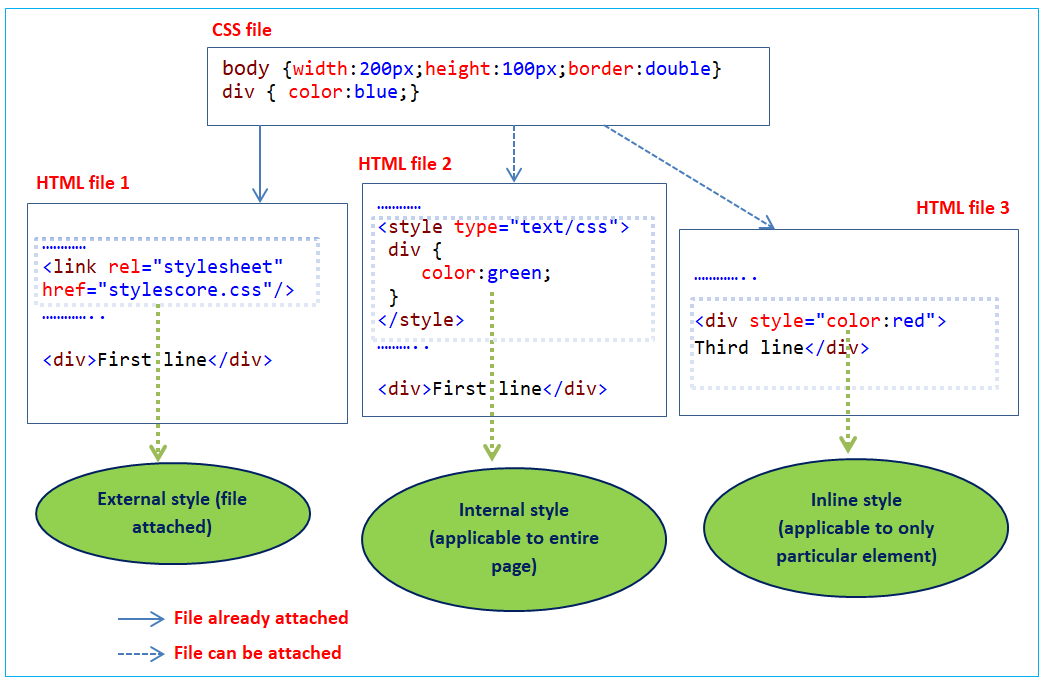
\includegraphics[width=1\textwidth]{classFiles/css_styling.png}
            \end{column}
        \end{columns}
    \end{tcolorbox}
\end{frame3}

\begin{frame4}
    \frametitle{Thank You}
\end{frame4}

\end{document}
